\section{Case Study}\label{ss:casestudy}

In this section, we present the results of applying our framework to investigate the potential benefits of static and dynamic personalization of apixaban dosing. Apixaban is a direct acting anticoagulant medication used to treat active blood clots occurring with deep venous thrombosis or pulmonary embolis, or to prevent stroke in patients with atrial fibrillation. Prescribing an apixaban dose that achieves blood concentrations within an optimal range is expected to provide optimal treatment benefits while minimizing harms (e.g., serious bleeding) for a drug considered to have a narrow therapeutic index. Indeed, patient-related factors that would predict high blood concentrations of apixaban such as age>80 years-old, weight <60 kg and kidney dysfunction are clinical variables that are normally considered in initial drug dose decisions. Additionally, female sex, comedications and genetic factors contribute to higher circulating apixaban concentrations \cite{gulilat2020drug}. These patient-related variables only explain 35\% of the pharmacokinetic variability in apixaban, which serves as rationale for dynamic dose optimization supported by post-initiation blood concentration monitoring. 
\subsection{Bayesian Modelling}

To create the necessary model for apixaban personalization, we extend a previously proposed one-compartment Bayesian pharmacokinetic model \cite{pananos2020comparisons} to include fixed effects of covariates on pharmacokinetic parameters in order to incorporate baseline clinical information (age, sex, weight, and creatinine.)  Full details of the model structure are provided in Appendix~\ref{ap:appendix}. We fit the model to previously-collected data on apixaban concentration \cite{tirona2018apixaban} and then use the fitted model to simulate patients with known "ground truth" pharmacokinetic parameters as described previously. We then use this population of simulated patients in our experiments to explore different modes of dose personalization and their relative benefits.

\begin{figure}
	\centering
	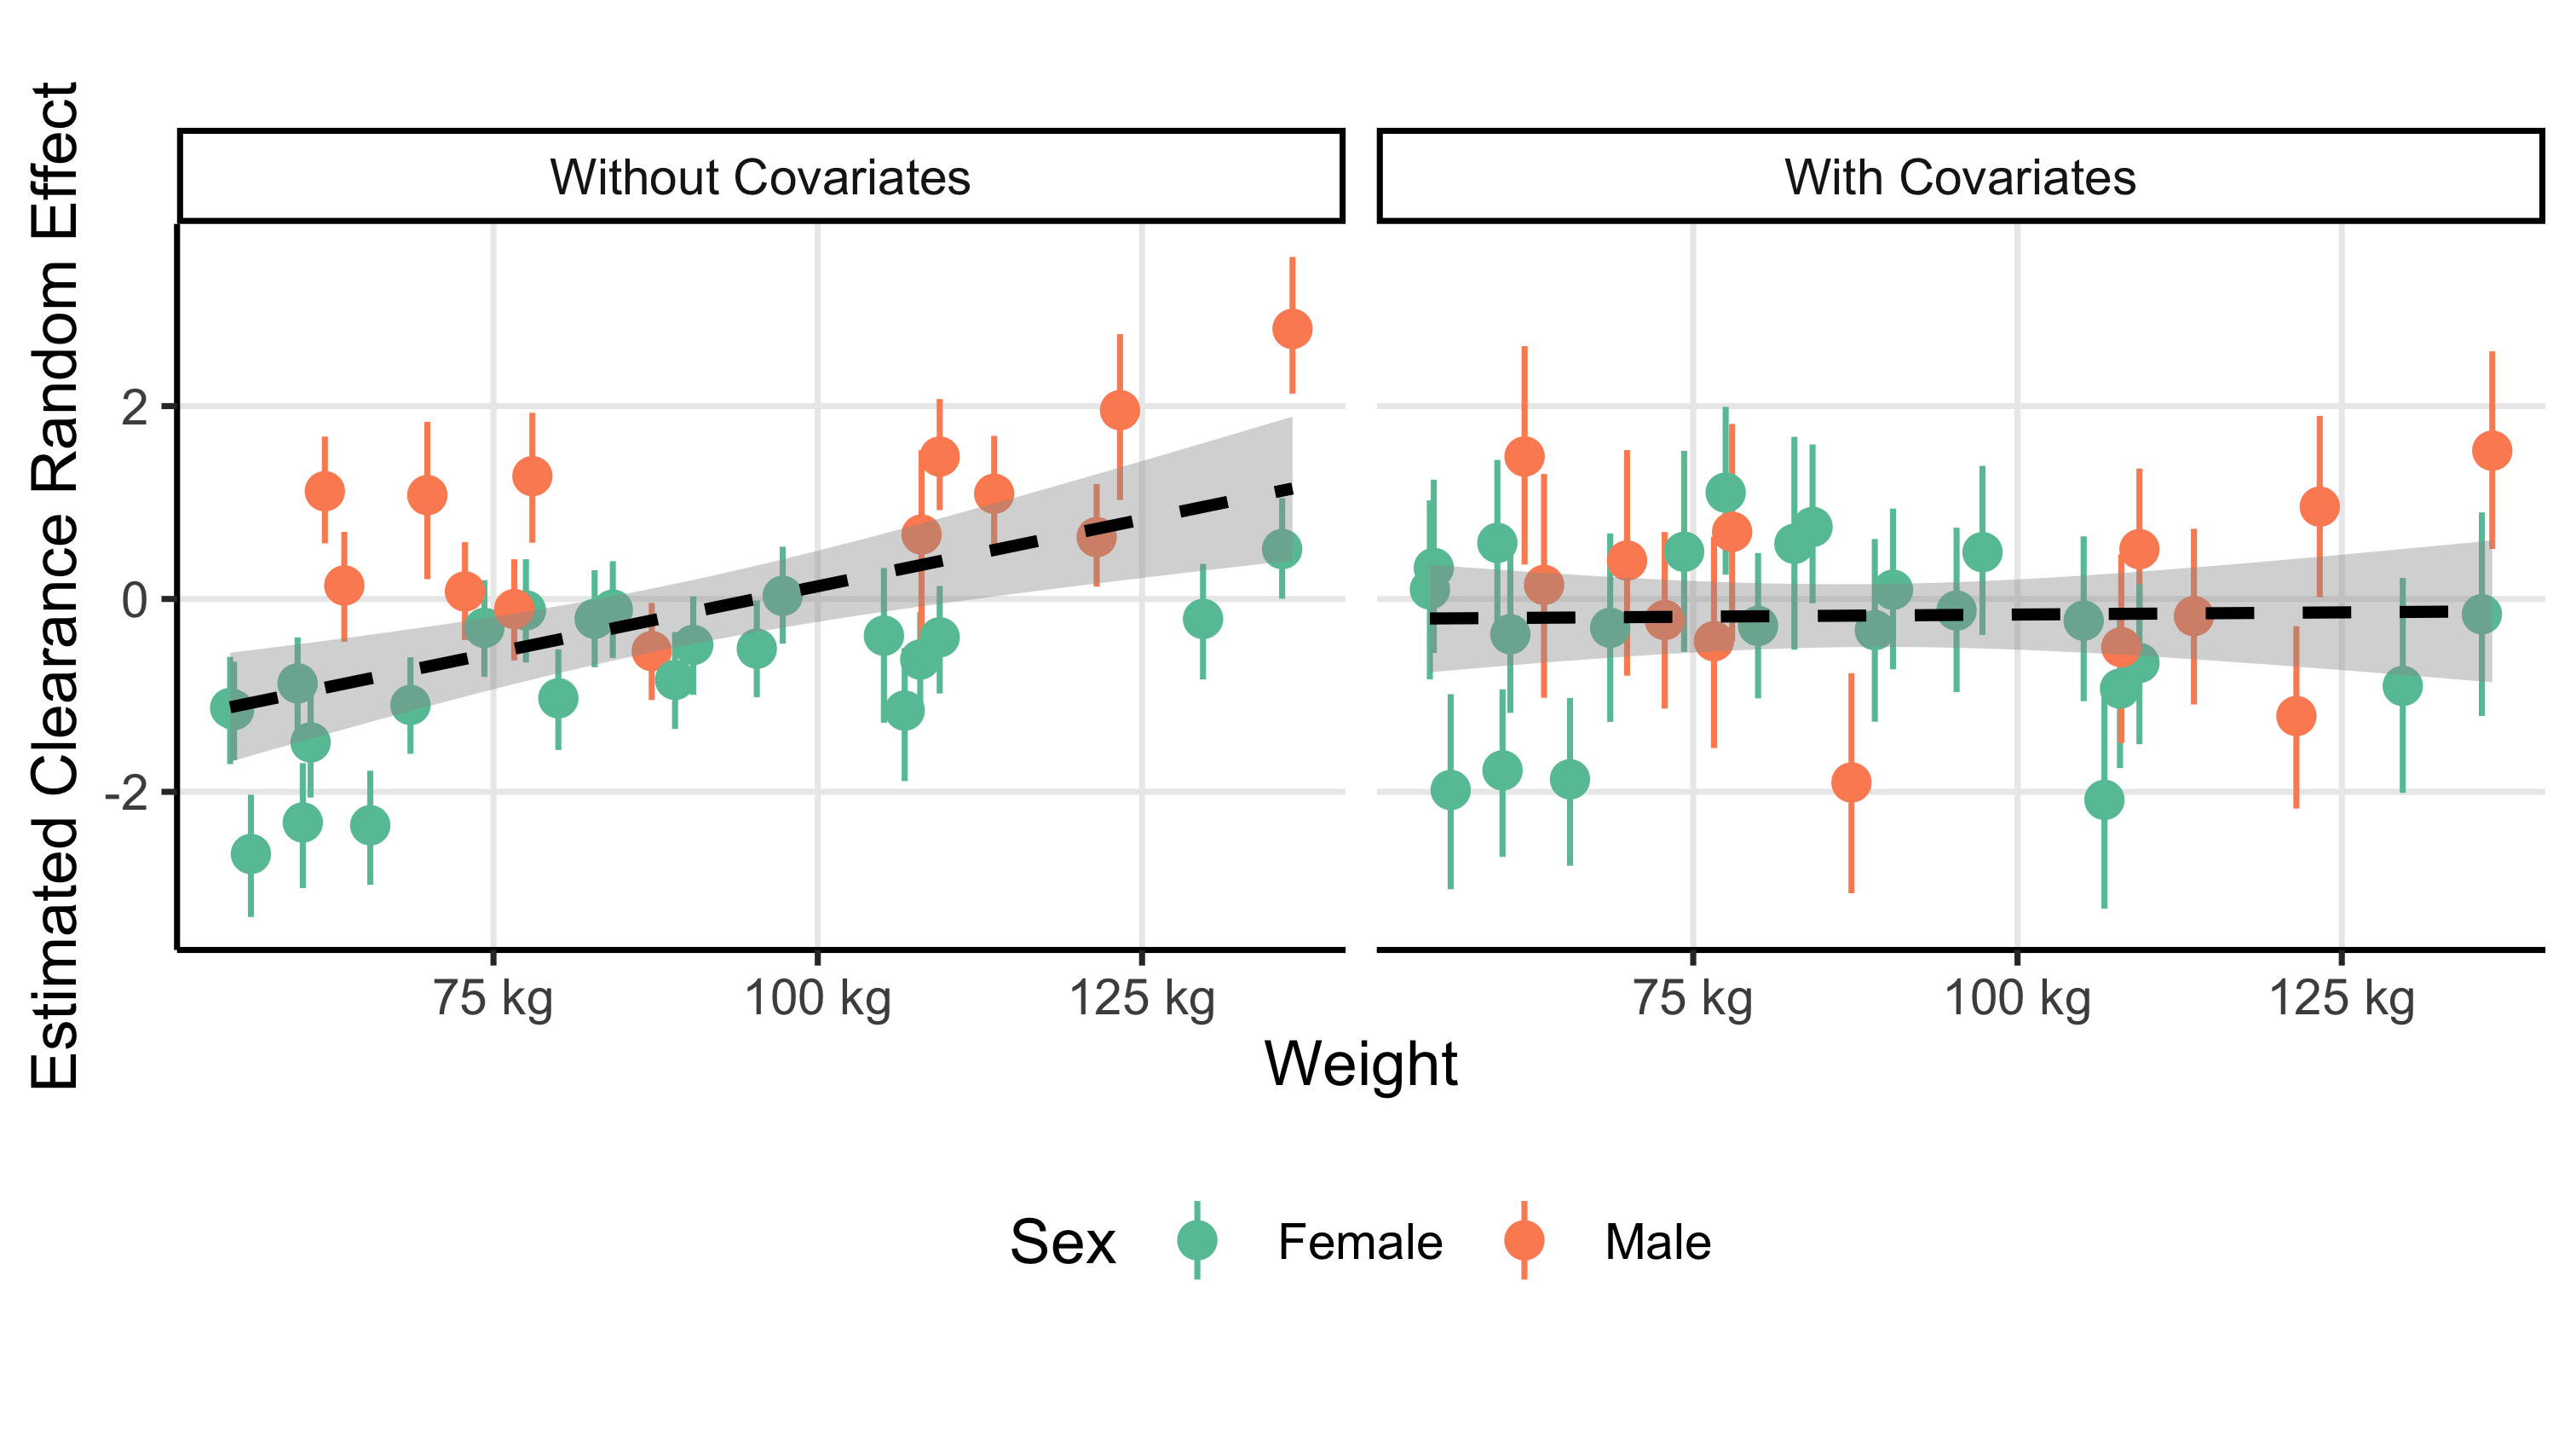
\includegraphics[width=\linewidth]{"figures/random_effects_change.png"}
	\caption{Random effects estimates for clearance $ CL_i $ and 95\% credible intervals (left).  Random effects estimates are colored by patient sex.  Prior to adjusting for covariates, a general trend in weight can be seen in the random effects.  Subjects who are heavier tend to have larger random effect, and males tend to have larger random effects than females of the same weight.  Patterns such as these indicate that weight and sex can be used to explain variation in the random effects.  After adjusting for sex and weight (right), the random effects have no discernable pattern.}
	\label{fig:randomeffectschange}
\end{figure}

We fit our model to real pharmacokinetic data using the open source probabalistic programming language, Stan \cite{gelman2015stan}.  Stan monitors several Markov chain diagnostics, none of which detected problematic Markov chain behavior, which indicates that Stan’s sampling algorithm was able to converge (0 divergences, all all Gelman-Rubin diagnostics<1.01, all effective sample size ratios  > 22\%).  

The inclusion of covariates in the model results in a better fit than excluding them. Shown in \cref{fig:randomeffectschange} are the estimated random effects for the clearance pharmacokinetic parameter of each subject as a function of weight.  Subject sex is indicated by color, the overall trend is shown in the black dashed line.  Failing to include subject sex and weight results in males having on average a larger random effect than females of the same weight, and heavier subjects having a larger random effect than lighter subjects.  When covariates are added into the model, the variation in the random effects attenuates, resulting in closer alignment to model assumptions. A better fit to the data means data generated from the model may be closer aligned with the true data generating process.

Examining the posterior distributions of the regression coefficients provides further insights into the relationships between covariates and pharmacokinetics. Greater subject weight is associated with an increase in the expected value of alpha (which is used to compute the elimination and absorption rates in the first order one compartment PK model.  The parameter $ \alpha $ is the ratio of how fast the drug exits the central compartment  how fast the drug enters the central compartment) which impacts the time to maximum concentration after each dose.  There is an estimated effect of sex on $ \alpha $ (males have smaller alpha than females, meaning the drug leaves their central compartment slower or enters the central compartment quicker), however the uncertainty is large (estimated effect -0.2 on the logit scale, 95\% credible interval -0.53 to 0.15). See \cref{tab:coefs} in the Appendix for a full summary of the regression coefficients.


%\begin{figure}
%	\centering
%	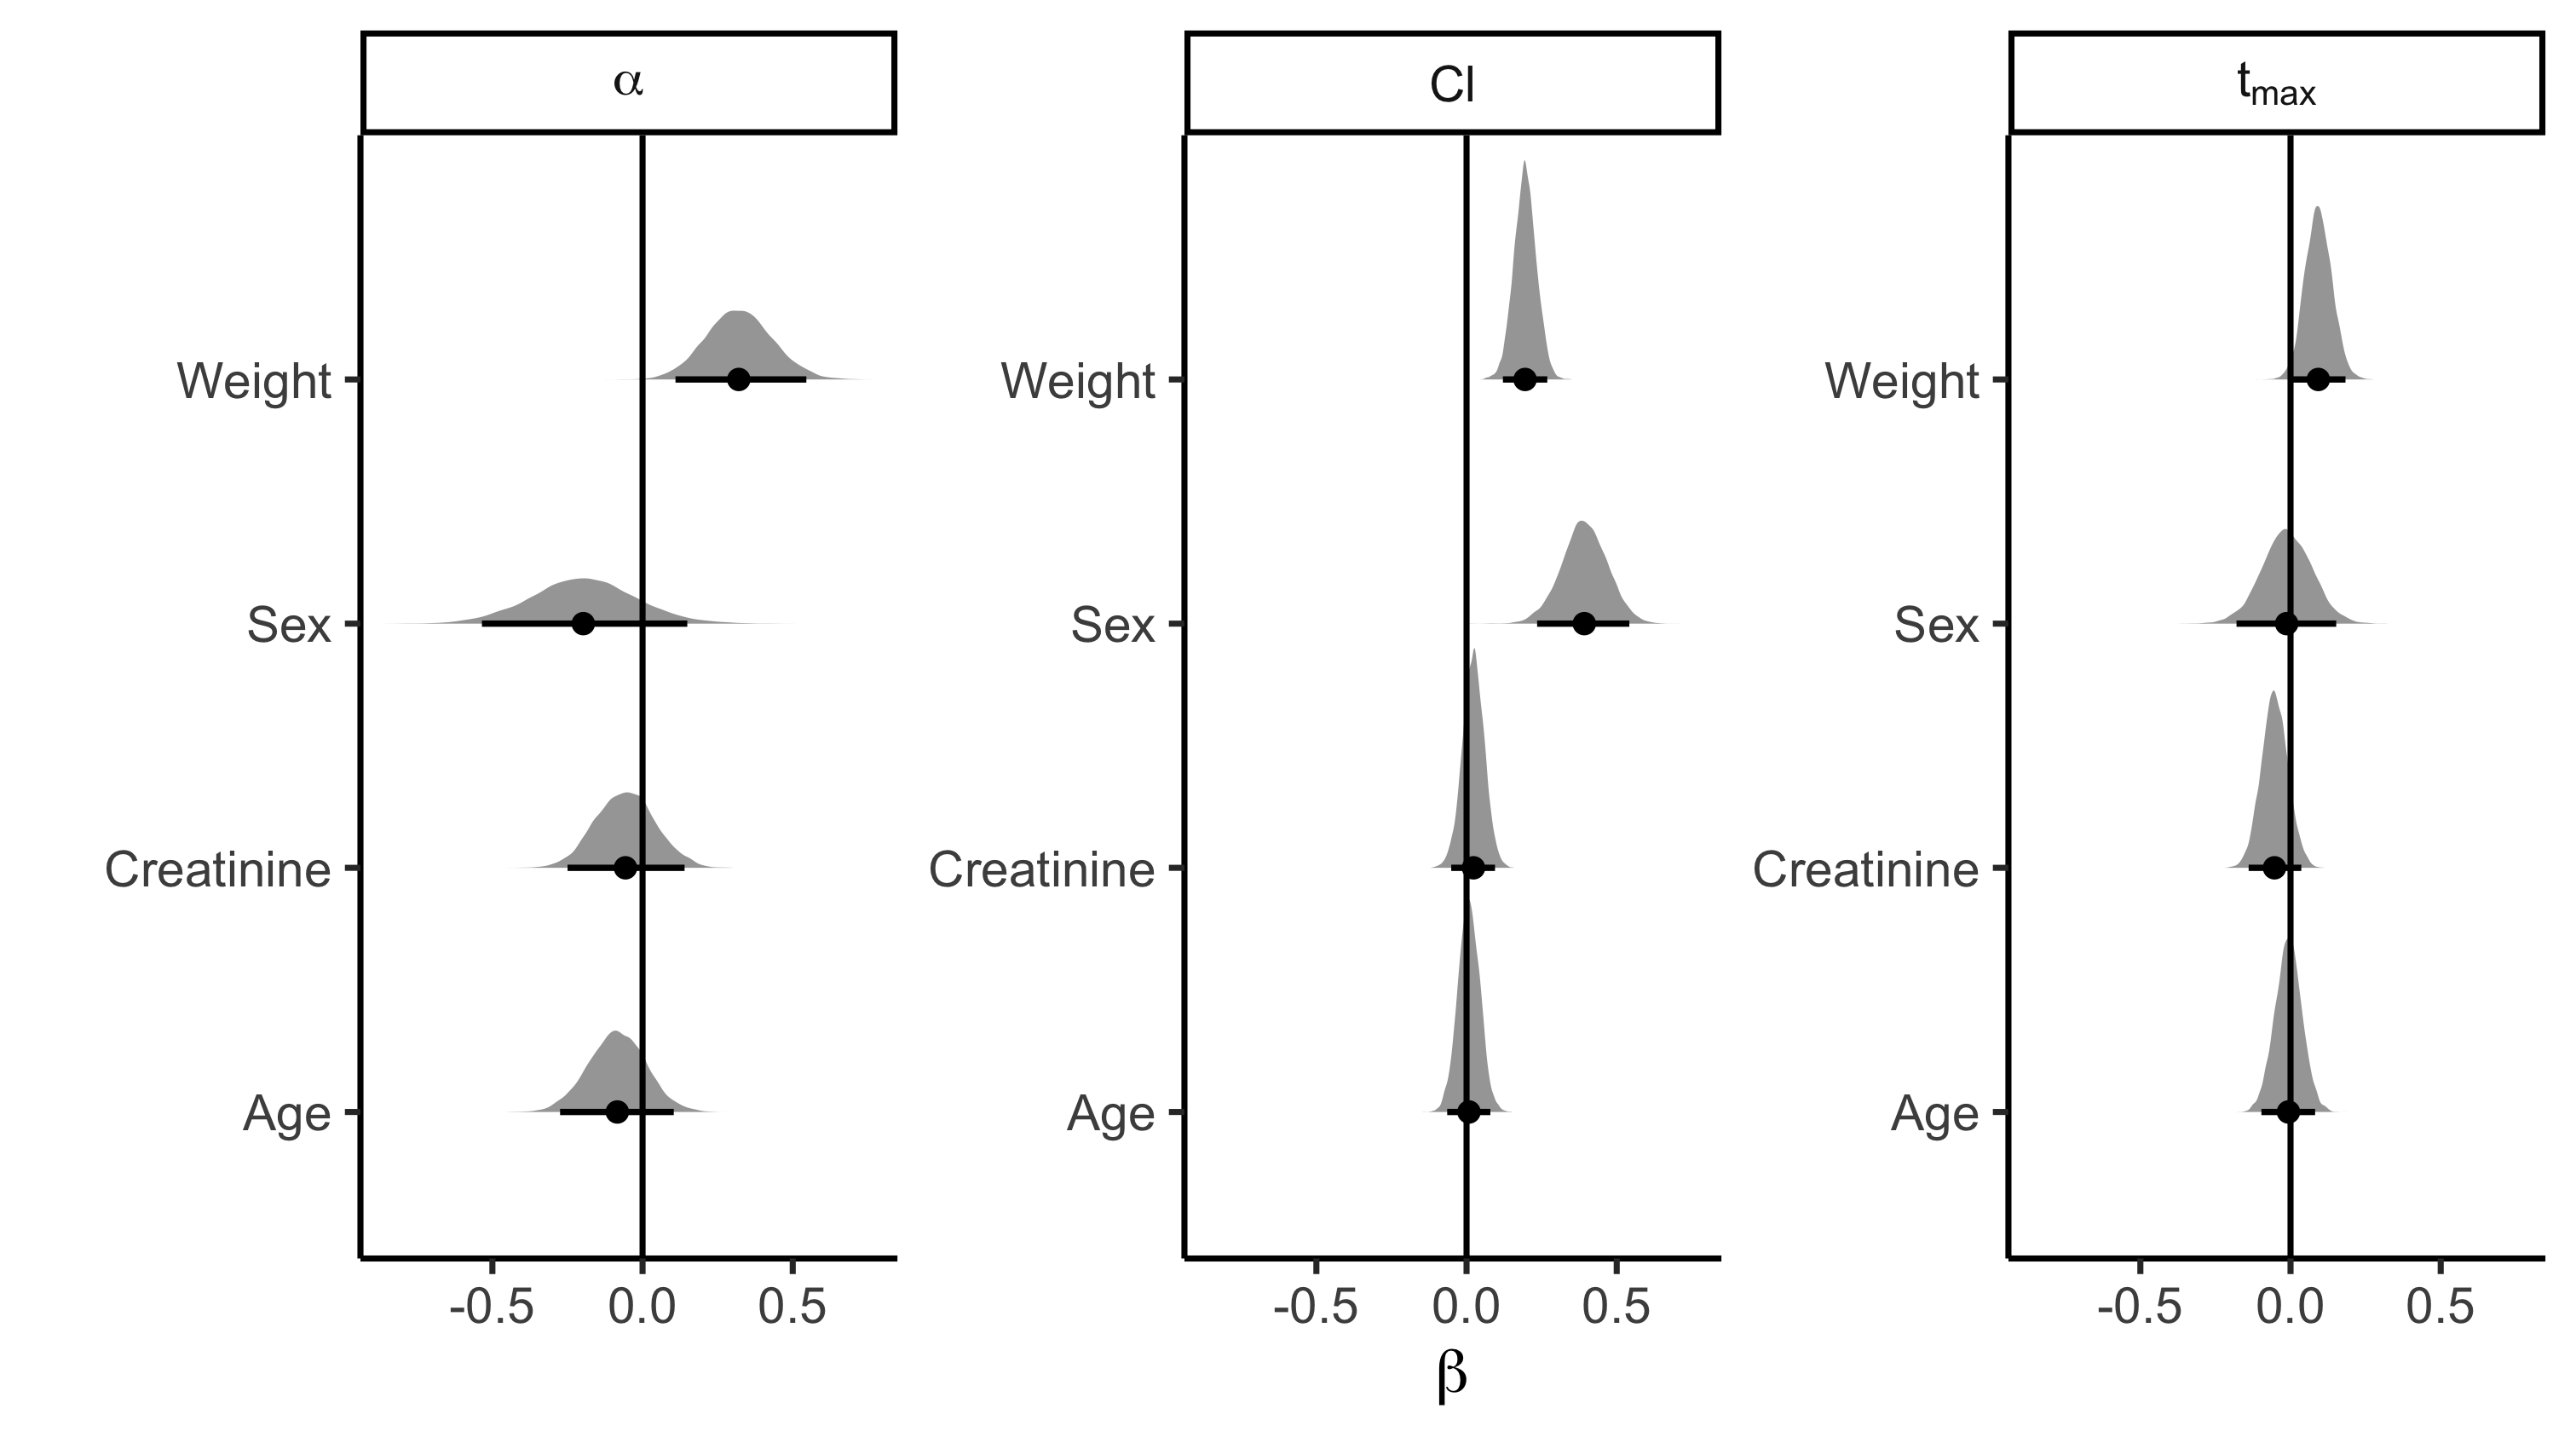
\includegraphics[width=1\linewidth]{figures/coef_vals}
%	\caption{Posterior distributions of regression coefficients. Expectations are shown as black dots, 95\% credible intervals are shown as horizontal black lines.  Solid black vertical line is $\beta=0$ for reference.  Note, regression coefficients for $Cl$ and $t_{max}$ act multiplicatively (a one unit increase in weight leads to a change in $Cl$ of $\exp(\beta)$), while regression coefficients for $\alpha$ are interpreted on the log odds scale.}
%	\label{fig:coefvals}
%\end{figure}


Model training error is comparable between the two models; the model without covariates achieves an average error of 8.31 ng/ml as measured by root mean squared error.  The model with covariates achieves a root mean squared error of 8.36  ng/ml.  Estimates of concentration uncertainty remain similar between the two models as well.  We conclude the inclusion of covariates in the model improves model inferences but does not substantially improve the fit of the model in this case.




\subsection{Modes of Personalization}



%\textcolor{red}{Make these descriptions "line up" with modes in Section 3? Break out into "static" and "dynamic"?}
%\begin{enumerate}[1)]
%\item Dose selection using a hierarchical Bayesian model which does not incorporate subject covariates.  This model was presented in Pananos \& Lizotte \cite{pananos2020comparisons}.  We refer to this mode as the “No Covariate Model”.
%\item 1) and conditioning the model on a single sample from the subject taken sometime in the final 12 hours before the half way point.  At the start of the fifth day, a new dose is selected and used for the remaining time.  We refer to this mode as “No Covariate + 1 Sample”.
%\item Dose selection from M2.  A single dose is selected at the start of the regimen and is used throughout the 10 simulated days. We refer to this mode as “Covariate Model”.
%\item 3) and conditioning the model on a single sample from the subject taken sometime in the final 12 hours before the half way point.  At the start of the fifth day, a new dose is selected and used for the remaining time. We refer to this mode as “Covariate model + 1 Sample”.
%\item A two stage DTR, however the initial dose is the result of the procedure in 3).  The best time to sample the patient is then determined via Q learning. We refer to this mode as “Optimal Sampling Time”.
%\item A two stage DTR estimated via Q learning.  We refer to this mode as “Q Learning”.
%\end{enumerate}

We consider the  6 modes of personalization as outlined in \cref{ss:framework}.  To evaluate these modes of personalization, we generate 1000 simulated subjects taking a dose of apixaban once every 12 hours with perfect adherence for a total of 10 days. The goal is to maximize the time spent with blood concentration level between between 100 ng/ml and 300 ng/ml. We choose this range as it is not so narrow that even optimal doses perform poorly, but not so wide that any dose can achieve high reward. For static modes of personalization, the selected initial dose is fixed over the 10 day period. For dynamic modes of personalization, some time in the second 12 hour period on the fourth day (between 108 and 120 hours after the initial dose), the simulated subject’s blood concentration is measured, and then at the start of the fifth day, the dose is adjusted based on all the pre-dose clinical measurements plus the observed concentration by incorporating information into the Bayesian model. 

\subsubsection{Defining the Dynamic Treatment Regimes}

To implement the two dynamic modes of personalization, we estimate DTRs with two stages (the first five days, and the latter five days).  For the dynamic personalization policies our experiments, we develop a DTR for selecting the best dose for keeping a patient’s blood plasma concentration within a desired range.  In terms of the DTR, the system is the patient for whom a dose is selected, the actions correspond to selection of dose sizes (and a time in the future to sample the patient, should the DTR require that), and the reward is the proportion of time spent within the desired concentration range. The trajectories we will use to estimate the optimal Q functions are of the form

\begin{equation}\label{key}
O_1, A_1, Y_1, O_2, A_2, Y_2
\end{equation}

\noindent The interpretation of a given trajectory is:
\begin{itemize}
	\item $ O_1 $ is any pre-dose clinical measurements of the subject.  In our experiments, we consider age in years, renal function (as measured by serum creatinine in mMol/L), weight in kilograms, and dichotmous biological sex (dummy coded so that male=1 and female=0).  We choose these variables as they are known to affect the pharmacokinetics of apixaban \cite{byon2019apixaban}.  
	\item $ A_1 $ is the initial dose to provide the subject.  If the DTR allows us to specify a time in the future at which to measure the subject’s blood serum concentration, then $A_1$ is the dual action of initial dose plus a time in the future at which to measure.
	\item $ Y_1 $ is the proportion of time spent within the concentration range in the first five days.
	\item $ O_2 $ is the pre clinical measurements of the subject plus the observed concentration made on the fourth day.
	\item $ A_2 $ is the dose adjustment
	\item $ Y_2 $ is the proportion of time spent within the concentration range in the final five days after the dose adjustment.
\end{itemize}

The actions $A_j$ effect the reward $Y_j$ by directly changing the concentrations at a given time.  For example, a larger dose will elicit larger concentrations which may put the patient in range for longer (more reward) or make take them out of range for some time (less reward).  Thus, our reward function can be thought of as a composition of the reward function and the concentration function.  In our experiments, we create a mesh of $2K$ times at which we can evaluate the latent concentration and compute the reward function.  Each stage in our DTR consists of $K=240$ times (equivalent to evaluating the latent concentration function every 30 minutes after ingestion).  Let $ c_i \>,  i=1...2K \>, $ be the $ i^{th}$ latent concentration value at time $ t_i $.  The reward function in the first stage is

\begin{equation}
Y_1(H_1, A_1) = Y_1(c_1(A_1), \dots, c_K(A_1)) = \dfrac{1}{K}\sum_{i=1}^K \mathbb{I}(0.1 < c_i(A_1) < 0.3)
\end{equation}



\noindent Here, $ \mathbb{I} $ is an indicator function returning 1 if $c_i$ is between 100 ng/ml and 300 ng/ml and 0 else.
%To leverage off-the-shelf optimization tools, we approximate this reward function with a continuously differentiable function, namely
%\begin{equation}
%Y(c_1, c_2, \cdots,  c_k) = \dfrac{1}{k}\sum_{j=1}^K \exp\left( - \left[ \dfrac{c_j-0.15}{0.05} \right]^{2\beta} \right)
%\end{equation}
%
%\noindent Here, $ \beta $is a positive integer.  For sufficiently large beta, our approximation becomes arbitrarily close to our intended reward function.  In practice we set beta=5 to balance between good approximation of our intended reward and vanishing gradients impeding our optimization. 
%We suppress the dependence on the history in the definition of the reward as the reliance on the history is implicit.  The reward depends on the latent concentrations which depend on previous doses (actions) and potentially on the previous dose measurements (observations of the system).  We approximate this reward function with a continuously differentiable function to facilitate optimization.  See the appendix for details.  
\noindent The reward function in the second stage is

\begin{equation}
Y_2(H_2, A_2) = Y_1(c_{K+1}(A_2), \dots, c_{2K}(A_2)) = \dfrac{1}{K}\sum_{i=1}^K \mathbb{I}(0.1 < c_{K+i}(A_2) < 0.3)
\end{equation}



Our stage 2 optimal Q function is then

\begin{equation}
Q_{2}^{o p t}\left(H_{2}, A_{2}\right)=E\left[Y_2\left(c_{K+1}(A_2), \cdots, c_{2K}(A_2)\right) \Bigg\vert H_{2}, A_{2}\right] \>,
\end{equation}

\noindent and our stage 1 optimal Q function is

\begin{equation}
Q_{1}^{o p t}\left(H_{1}, A_{1}\right)= E \left[Y_1\left(c_{1}(A_1),  \cdots, c_{K}(A_1)\right)+\max _{a_{2} \in \mathscr{A}} Q_{2}^{o p t}\left(H_{2}, a_{2}\right) \Bigg\vert H_{1}, A_{1}\right]
\end{equation}

We seek to maximize the stage 1 optimal Q function to learn the optimal policy for dosing subjects under the constraint we can measure them at most once and are limited to the aforementioned pre-dose clinical variables.  The interpretation of stage 1 optimal Q function is as follows:\textit{ Given the pre-dose clinical variables of the subject and a proposed initial dose and measurement time, the stage 1 optimal Q function gives the proportion of time the subject’s blood serum concentration is between 100 ng/ml and 300 ng/ml assuming that we provide the subject with the best dose possible at the start of the $ 5^{th} $ day.}  The actions $ A_1 $ and $ A_2 $ which maximize these functions constitute the optimal policy.


%
%The concentration values $ c_j $ in the optimal Q functions are latent, meaning we have no direct access to them in practice. Furthermore, obtaining measurements with high enough frequency so that the reward is faithfully estimated would be too burdensome on the patient. 


\subsection{Evaluation}

We present the results of our simulation in \cref{fig:modelsofpersonalizationdifferences} below in terms of difference between theoretically largest return and achieved return by each mode of personalization.  The results are ordered from least amount of information and burden (top) to most amount of information and burden (bottom) and colored by their personalization strategy (static or dynamic).

Modes of personalization which use less information have a larger difference (i.e. yield smaller return on average than what is theoretically possible).  The One Size Fits All approach (which uses no information about the subject) performs worst with a median difference of 0.145.  The distribution of differences for this mode is right skewed with some differences exceeding 0.95, meaning the subject could have been in range for nearly the entire time but the mode selected a dose which failed to put the subject in range. 

The use of clinical variables in the model nearly cuts the difference in half, achieving a median difference of 0.086 with smaller right skew.  There is a diminishing in the difference in returns as additional burden is undertaken. Modes which use observed concentration information (Clinical Variables + One Sample, Optimal Sampling Time, and Optimal Sequential Dosing) lead to marginally lower median differences  (0.075, 0.076, 0.079 respectively) as compared to the use of clinical variables alone.


\begin{figure}
	\centering
	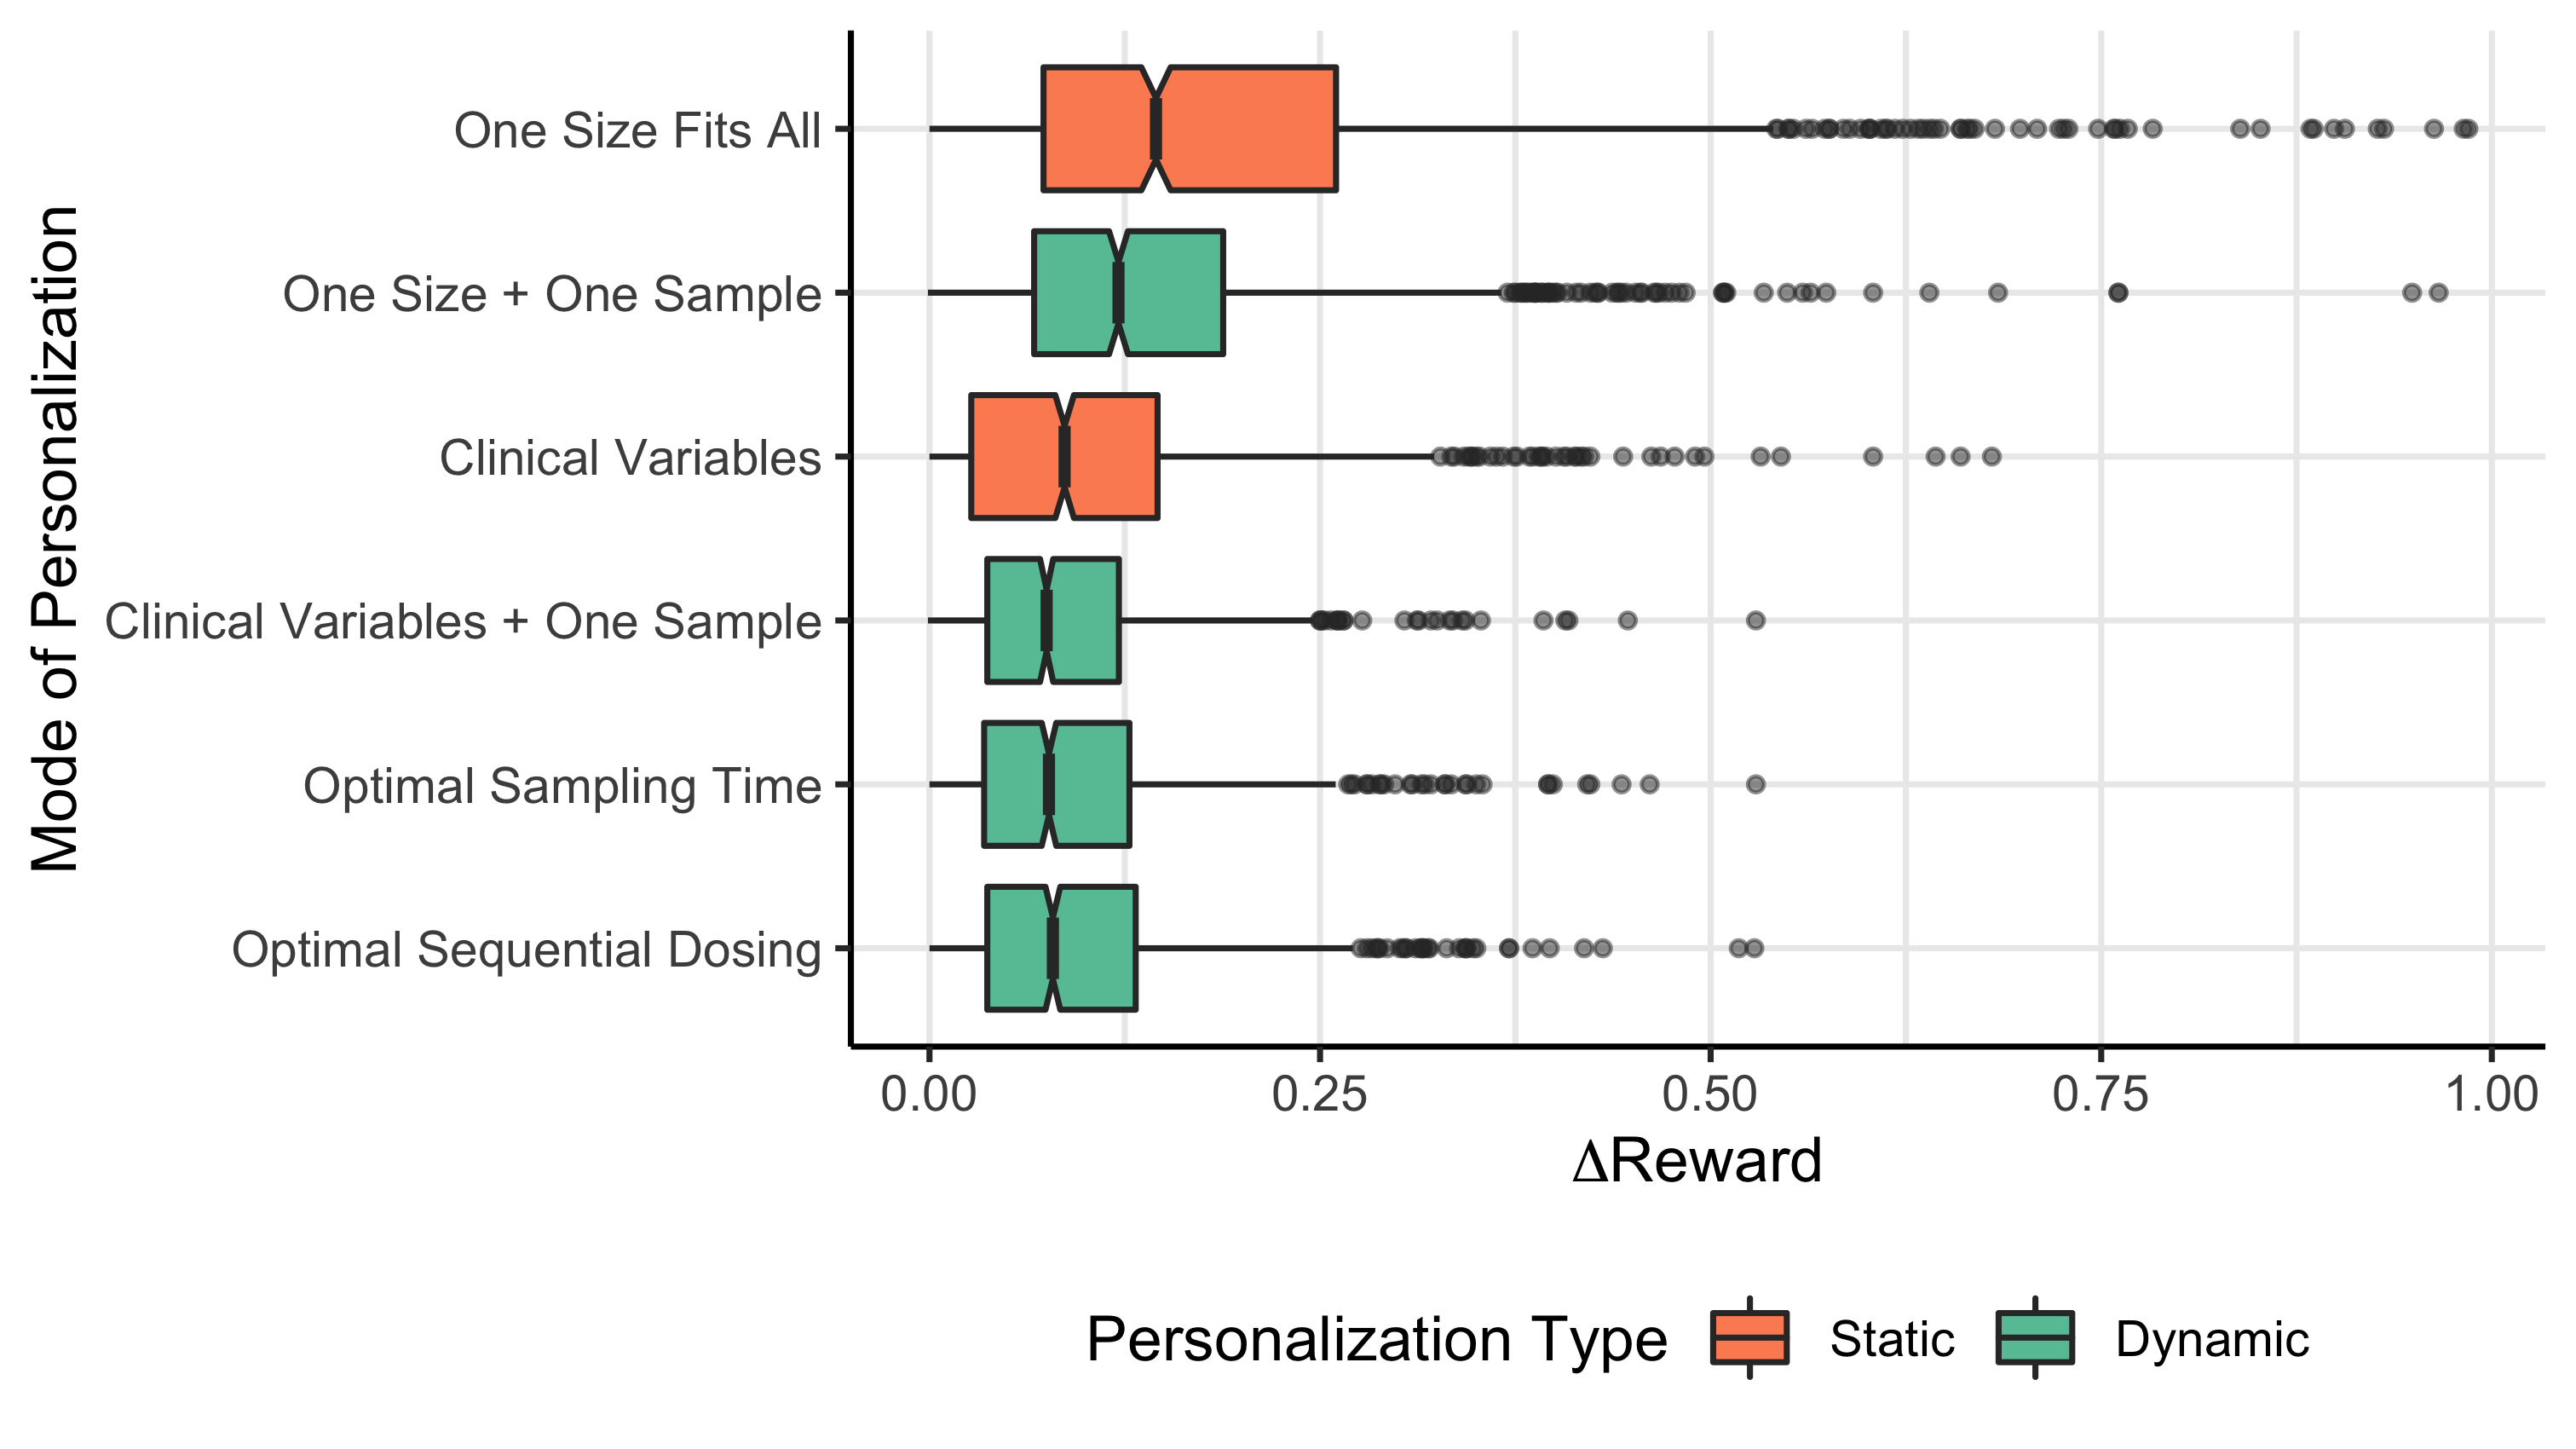
\includegraphics[width=1\linewidth]{figures/models_of_personalization_differences}
	\caption{Boxplots of the difference between theoretically largest return and achieved return for each of the 1000 simulated subjects. Subjects who achieve a reward close to their maximium return have a difference on 0, subjects who achieve a return less than their maximum have larger differences, with the largest difference being 1.}
	\label{fig:modelsofpersonalizationdifferences}
\end{figure}
